
\documentclass[a4paper,11pt]{article}
\usepackage[margin=1.5cm]{geometry}
\usepackage{graphicx}
\usepackage{amsmath}
\usepackage{booktabs}
\usepackage{setspace}
\usepackage{microtype}
\pagenumbering{gobble}
\begin{document}

\begin{center}
\Large\textbf{Is Florida Getting Warmer?}\\[4pt]
\normalsize Permutation Test on Key West Annual Mean Temperature (20th Century)
\end{center}

\vspace{0.5cm}

\section*{1. Methods}
Annual mean temperatures recorded at Key West, Florida, were correlated with year. 
Let $r_{\text{obs}}$ be the observed Pearson correlation coefficient:
\[
r_{\text{obs}} = 0.5332
\]
To test whether this correlation is greater than expected by chance, 
temperatures were randomly shuffled among years $N = 10000$ times, and the correlation recalculated each time:
\[
r_i = \text{cor}(\text{Year}, \text{sample(Temp)})
\]
The empirical p-value is computed as the fraction of permuted correlations greater than or equal to the observed one:
\[
p = \frac{\sum (r_i \ge r_{\text{obs}})}{N} = 0.0000
\]

\section*{2. Results}
The histogram below shows the distribution of correlation coefficients from the permutation test. 
The vertical red line marks the observed correlation $r_{\text{obs}}$.

\begin{center}
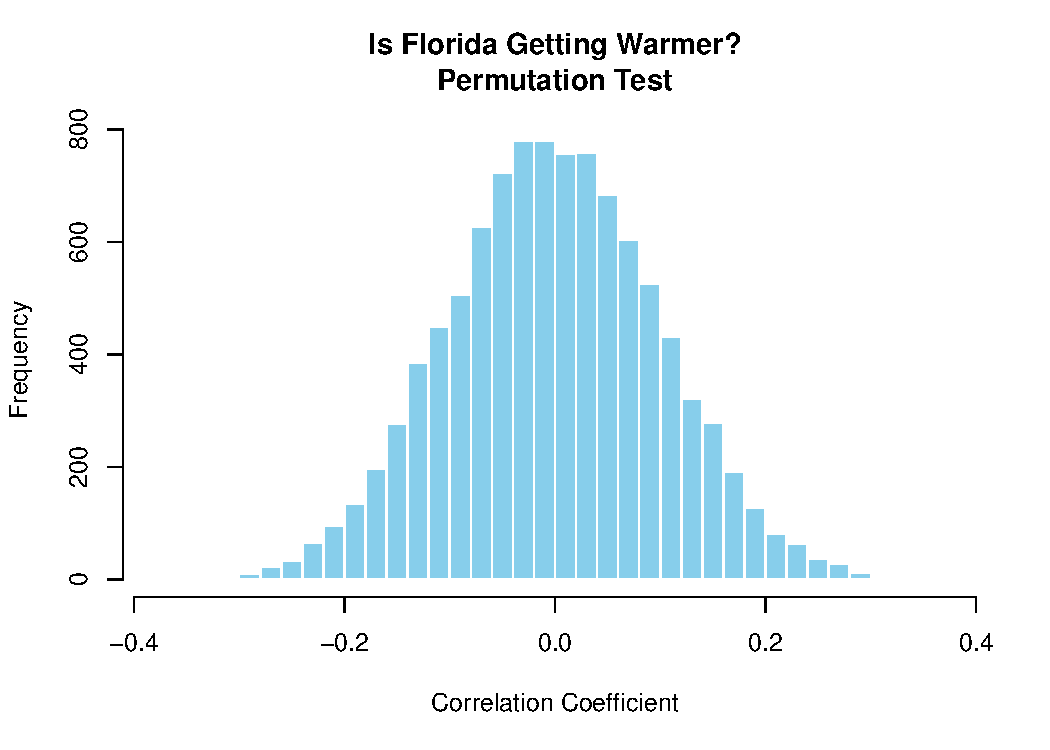
\includegraphics[width=0.9\textwidth]{Florida_histogram.pdf}
\end{center}

\vspace{0.3cm}
\noindent
\textbf{Observed correlation:} $r = 0.5332$\\
\textbf{Empirical p-value:} $p = 0.0000$\\
\textbf{Number of permutations:} $N = 10000$

\vfill
\noindent\textit{Generated automatically by Florida.R (R version 4.5.1).}
\end{document}

